% Graph paper
% Author: Benjamin Abel
% Fibonacci spiral
% Author: Andrew Mertz
\documentclass{article}
\usepackage{geometry}
\geometry{hmargin=1cm,vmargin=1cm}
\usepackage{amsmath,tikz}
\def\width{19}
\def\hauteur{12}

\usetikzlibrary{backgrounds,calc}

\begin{document}

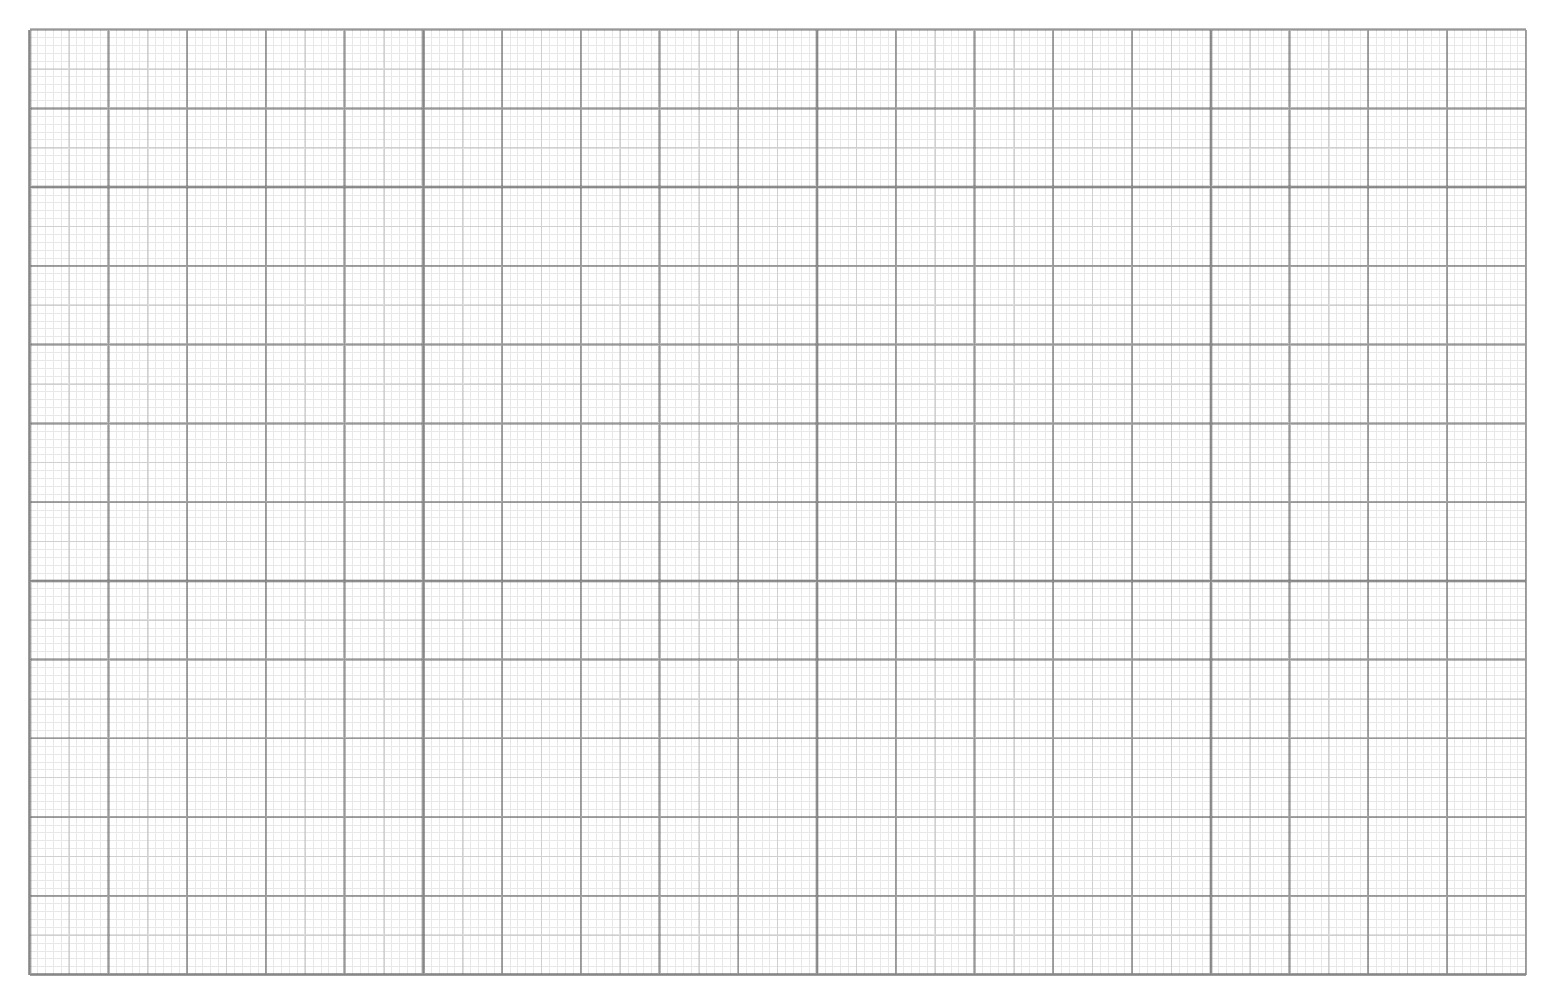
\begin{tikzpicture}[x=1cm, y=1cm, opacity=0.3]
\draw[step=1mm, line width=0.1mm, black!30!white] (0,0) grid (\width,\hauteur);
\draw[step=5mm, line width=0.2mm, black!40!white] (0,0) grid (\width,\hauteur);
\draw[step=5cm, line width=0.5mm, black!50!white] (0,0) grid (\width,\hauteur);
\draw[step=1cm, line width=0.3mm, black!90!white] (0,0) grid (\width,\hauteur);
\end{tikzpicture}

\begin{tikzpicture}[scale=1.293,x=1cm, y=1cm, opacity=0.2, overlay]
  % Create some counters for holding the Fibonacci numbers
  \newcounter{a}
  \newcounter{b}
  \newcounter{temp}

  % Initialize the counters
  \setcounter{a}{0}
  \setcounter{b}{1}

  % The spiral will start at the origin
  \coordinate (0) at (10.64,2.87);

  % This loop defines the number of turns in the spiral. Note that we
  % will have to be careful not to overflow our counters or make the
  % spiral too large for TeX to handle. This is easy to do as the
  % Fibonacci sequence grows exponentially.
  \foreach \i in {1,...,18}
  {
    % Get the "name" of the last point on the spiral
    \pgfmathsetmacro{\lastpoint}{\i-1}

    % Compute the angle for this turn of the spiral
    \pgfmathsetmacro{\startangle}{mod(\i-1,4) * 90}

    % Draw this turn of the spiral and remember the point where we end
    \draw[black] (\lastpoint) arc
      (\startangle : \startangle + 90 : \value{b}/10.0pt) coordinate (\i);

   % Compute the next Fibonacci number
    \setcounter{temp}{\value{b}}
    \addtocounter{b}{\value{a}}
    \setcounter{a}{\value{temp}}
 }
\end{tikzpicture}

\end{document}

